\documentclass[tikz,border=10pt]{standalone}

\usepackage{xcolor}
\usetikzlibrary{arrows.meta, positioning}

\definecolor{paperGreen}{RGB}{34,125,92}
\definecolor{paperSoft}{RGB}{246,248,250}
\definecolor{paperLine}{RGB}{80,92,110}

\begin{document}
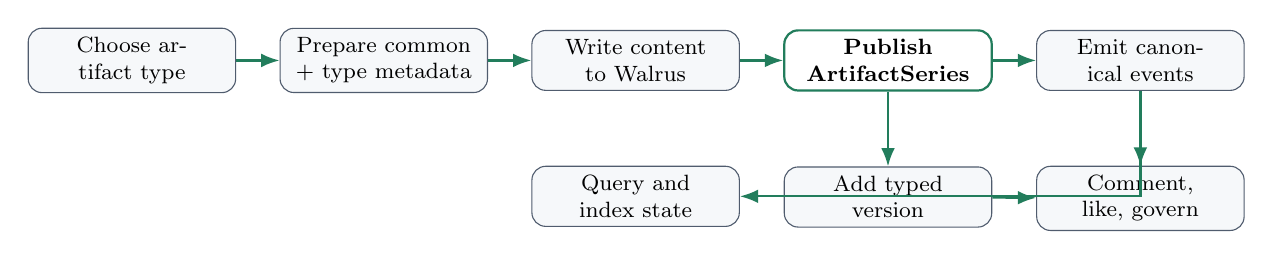
\begin{tikzpicture}[
    flowstep/.style={draw=paperLine, rounded corners=5pt, fill=paperSoft, minimum height=0.72cm, align=center, font=\footnotesize, text width=2.4cm},
    hot/.style={draw=paperGreen, thick, rounded corners=5pt, fill=white, minimum height=0.72cm, align=center, font=\footnotesize\bfseries, text width=2.4cm},
    arrow/.style={-Latex, thick, draw=paperGreen},
    node distance=0.55cm
]
    \node[flowstep] (type) {Choose artifact type};
    \node[flowstep, right=of type] (meta) {Prepare common + type metadata};
    \node[flowstep, right=of meta] (content) {Write content to Walrus};
    \node[hot, right=of content] (publish) {Publish ArtifactSeries};
    \node[flowstep, right=of publish] (events) {Emit canonical events};
    \node[flowstep, below=0.95cm of publish] (addv) {Add typed version};
    \node[flowstep, below=0.95cm of events] (interact) {Comment, like, govern};
    \node[flowstep, below=0.95cm of content] (query) {Query and index state};

    \draw[arrow] (type) -- (meta);
    \draw[arrow] (meta) -- (content);
    \draw[arrow] (content) -- (publish);
    \draw[arrow] (publish) -- (events);
    \draw[arrow] (publish) -- (addv);
    \draw[arrow] (events) -- (interact);
    \draw[arrow] (events) |- (query);
    \draw[arrow] (addv) -- (interact);
\end{tikzpicture}
\end{document}
